%!TEX root=../GaugeCNNTheory.tex


\subsection{Rotation-steerable surface convolutions}
\label{sec:so2_surface_conv}

In this section we review the $\SO2$, $\CN$ and $\DN$-steerable surface convolutions that are listed in  rows (37-40) of Table~\ref{tab:network_instantiations}.
All of these models have in common that they address the ambiguity of reference directions on general surfaces via a locally rotation equivariant (or invariant) design, which distinguishes them from the $\{e\}$-steerable models discussed in the following Section~\ref{sec:e_surface_conv}.
Before discussing the individual models in detail, we start with a higher level overview of common design choices and possible numerical discretizations.


\paragraph{General remarks and overview:}
All of the models that are reviewed in this section operate on \emph{triangle surface meshes} and are rotation-steerable.
The continuous structure group $G=\SO2$ is for all models that assume regular field representations (rows (38) and (39)) discretized by cyclic groups~$\CN$, i.e. $N$ equally spaced directions.
The model by \citet{huang2019texturenet} assumes a more specific structure group $\D4$.
Note that the purely rotation-steerable architectures operate only on \emph{oriented surfaces} without violating the smoothness (continuity) of their inference.
Non-oriented surfaces require additional reflection-steerability, i.e. structure groups $\O2$ or $\DN$.
This requirement is often easily satisfiable with minor adaptations, most importantly by using further restricted kernel spaces.


In accordance with the definition of $\GM$-convolutions, the models parameterize features in the local neighborhood around each sampling point in terms of \emph{geodesic normal coordinates}.
Almost all of the models sample feature fields on the \emph{mesh vertices}; only \citet{huang2019texturenet} samples features densely on the mesh faces.
The continuous convolution integral in Eq.~\eqref{eq:gauge_conv_coord_expression}, which matches the features in geodesic normal coordinates with a steerable kernel, can be discretized in different ways.
The majority of models discretize this integral at a vertex $p\in\mathcal{V}$ as a summation over its neighboring vertices $\mathcal{N}_p \subset \mathcal{V}$.
Features from these vertices $q\in\mathcal{N}_p$ are then matched with the values of the continuous kernel at point $\psiTMp \log_p(q) \in \R^2$, where $\psiTMp^A$ is the gauge corresponding to the chosen reference frame at~$p$.
Together with the transport from $q$ to $p$, this results in the discretization
\begin{align}\label{eq:mesh_conv_neighbor_log_discretization}
    \fout^A(p)\ =\ \sum_{q\in\mathcal{N}_p} \textup{A}_q\, K\big(\psiTMp^A \log_p(q)\big)\, \rho\big( g^{A\widetilde{A}}_{p\leftarrow q} \big)\, \fin^{\widetilde{A}}(q) \,,
\end{align}
where $\textup{A}_q \in \R$ are suitably chosen area weights that sum to the total mesh area, ${\sum_{q\in\mathcal{V}} \textup{A}_q = \int_M 1 dp}$.
Common choices are barycentric area weights of the form
\begin{align}\label{eq:triangle_area_weights}
    w_q = \frac{1}{3} \sum_{\{i,j,q\}\in\mathcal{F}} A_{\{i,j,q\}} \,,
\end{align}
with the sum running over all triangles that are adjacent to vertex~$q$, or Voronoi areas~\cite{vouga2014lectures}.
Since the discretization in Eq.~\eqref{eq:mesh_conv_neighbor_log_discretization} sums over neighboring vertices, the algorithms compute log maps via \emph{shortest geodesics} between $q$ and~$p$; see Section~\ref{sec:surfaces_geom_mesh} and~\cite{polthier1998straightest}.

Instead of computing logarithmic maps of neighboring vertices, one can alternatively discretize the convolution integral on the kernel domain~$\R^2$.
The authors of \cite{masci2015geodesic} use an equiangular and equiradial binning of geodesic polar coordinates.
They compute the exponential map for each sampling point $(r,\varphi)$, that is, they shoot a \emph{straightest geodesic} (\cite{polthier1998straightest}) of length $r$ in direction $\varphi$ relative to the reference frame.
As these geodesics end in general in a face, the feature vectors from adjacent vertices need to be interpolated, 
for instance based on barycentric coordinates.
\citet{Yang2020parallelFrameCNN} approximate the geodesic neighborhood via a ``parallel transport unfolding'' algorithm~\cite{budninskiy2018parallel}.


Table~\ref{tab:network_instantiations} organizes the models by their respective \emph{field types}, i.e. by the group representations $\rho$ that specify their transformation laws under gauge transformations.
The only non-trivial field types used so far are (complex) \emph{irreducible representations} of $\SO2$ \cite{Wiersma2020} and \emph{regular representations} of $\SO2$, discretized by regular representations of a discrete subgroup $\CN$~\cite{poulenard2018multi,sun2018zernet,deHaan2020meshCNNs,Yang2020parallelFrameCNN}.
Regular representations of $\SO2$ act by definition on functions on $L^2(\SO2)$, that is, on features which assign ``one value per direction''.
In the discretized version, we have $L^2(\CN) \cong \R^{|\CN|} = \R^N$, where each of the $N$~dimensions of a regular feature vector corresponds to one of the directions in~$\big\{ k\frac{2\pi}{N} \big|\, k=0,\dots,N-1 \big\}$.
The correspondence to regular representations is in most of these papers implicit -- the network architectures are rather derived from a more intuitive viewpoint.
It turns out that the authors use only a subset of the complete space of steerable kernels that map between $\CN$-regular feature fields.
We substantiate this claim further below when discussing the models in detail.
A construction of the complete kernel space is given in \cite{Weiler2019_E2CNN}, a visualization can be found in Fig.~3 of~\cite{Weiler2018SFCNN}.
The remaining models are based on \emph{trivial representations}, i.e. \emph{scalar fields}.
One approach to compute scalar fields is to apply a kernel in $N$ directions, resulting in an intermediate $\CN$-regular feature field, followed by a pooling operation over the $N$ responses~\cite{masci2015geodesic,monti2017geometric,sun2018zernet}.
Since gauge transformations in $\CN$ will lead to a mere cyclic shift (a permutation) of the feature's direction channels, the pooling operations are \emph{invariant} under gauge transformations, i.e. result in scalar fields.
\citet{huang2019texturenet} uses immediately $\D4$-invariant kernels; see Fig.~\ref{fig:3x3_D4_invariant_kernel}.
As gauge transformation leave such kernels invariant, the resulting feature fields are invariant as well, i.e. scalar fields.


Lastly, we can compare the models by the \emph{feature transporters} that they assume.
All of the convolutional networks in \cite{Wiersma2020,poulenard2018multi,sun2018zernet,deHaan2020meshCNNs} assume the canonical \emph{Levi-Civita} transporters on the mesh.
As all of the models in \cite{masci2015geodesic,monti2017geometric,sun2018zernet,huang2019texturenet} rely on \emph{scalar fields} their parallel transport is trivial.
An alternative approach was followed by \citet{Yang2020parallelFrameCNN} who compute a $\CN$-valued connection on the mesh.
This connection is flat (trivial) everywhere except for at a few singularities with a holonomy of $k\frac{2\pi}{N}$ for some $k=0,\dots,N-1$ and fixed~$N$.
The authors optimize their $\CN$-valued connection such that it approximates the $\SO2$-valued Levi-Civita connection as close as possible; see also~\cite{craneTrivialConnectionsDiscrete2010}.
Note that this approach is similar to the local flattening of spherical CNNs into icosahedral CNNs ($N=6$) from Section~\ref{sec:spherical_CNNs_icosahedral} but applies to general meshes.




With these general remarks in mind, we focus on some more specific design choices that are made in the models.


\paragraph{Harmonic Surface Networks:}
The \emph{Harmonic Surface Networks} by \citet{Wiersma2020}, listed in row (37) of Table~\ref{tab:network_instantiations},
are a prototypical example of $\GM$-convolutions on meshes.
They generalize Harmonic Networks \cite{Worrall2017-HNET} -- whose features transform according to the complex irreps of $G=\SO2$ -- from the Euclidean plane to general curved spaces.
The authors define their convolution as in Eq.~\eqref{eq:mesh_conv_neighbor_log_discretization}, using the barycentric area weights from Eq.~\eqref{eq:triangle_area_weights}.
Levi-Civita transporters and logarithmic maps are computed via the vector heat method~\cite{Sharp2019VectorHeatMethod}, which is not restricted to triangle meshes but allows to apply the model to polygon meshes and point clouds.
The $\SO2$-equivariant nonlinearities used by the models act only on the absolute value of the complex features but leave their argument invariant.

As proven in \cite{lang2020WignerEckart,Weiler2019_E2CNN}, the $\SO2$-steerable kernel spaces that are used by the authors are complete over the complex field.
However, if the complex feature fields are implemented in terms of two channels that contain their real and complex parts, they should rather be viewed as transforming according to the real irreps of~$\SO2$.
The kernel constraint allows in this case for additional steerable kernels; see Appendix~F.5 of~\cite{Weiler2019_E2CNN} for a detailed discussion.
We furthermore want to mention that empirical evidence suggests that networks which are based on irrep fields perform significantly worse that those that are based on regular representations; see e.g. the benchmark in~\cite{Weiler2019_E2CNN}.
Note that Harmonic Surface Networks can easily be turned into networks that operate on regular feature fields by employing the ``regular nonlinearity'' from~\cite{deHaan2020meshCNNs}, which essentially applies a Fourier transformation of a stack of irrep fields to transform them into a regular feature field.


\begin{figure}
    \centering
    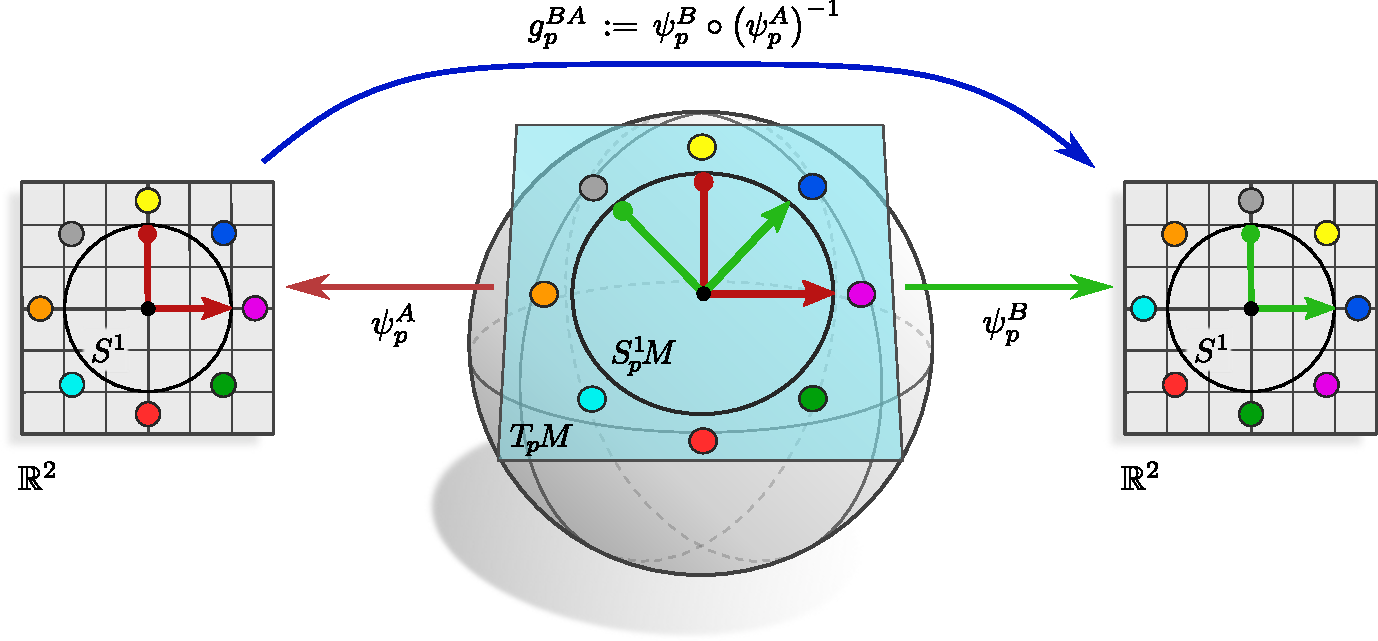
\includegraphics[width=1.\textwidth]{figures/directional_function.pdf}
    \caption{\small
        Visualization of the \emph{directional functions} by \citet{poulenard2018multi}.
        Directional functions assign a real-valued response (colored dots) to each direction (unit vector) in $\SpM \subset \TpM$ (black circle).
        When expressing these functions relative to right-handed, orthonormal reference frames or gauges $\psiTMp^X$, the coordinate representations assign real-valued responses to unit vectors in $S^1 \subset \R^2$.
        The transformation law between these coordinate representations is given by a rotation of the feature values on~$S^1$.
        Mathematically, this transformation law is identified as the action of the \emph{regular representation} of $\SO2$; see Eq.~\eqref{eq:directional_functions_trafo_law_regular}.
        Directional functions are therefore regular feature fields, and the surface CNN of \citet{poulenard2018multi} is based on $\GM$-convolutions between such fields.
        A diagrammatic version of this figure is given in Eq.~\eqref{cd:directional_function_trafo_law}.
    }
    \label{fig:directional_function}
\end{figure}


\paragraph{Multi Directional Geodesic CNNs:}
\citet{poulenard2018multi} proposed \emph{Multi Directional Geodesic CNNs} (MDGCNNs) which operate on so called \emph{directional functions}.
As we argue in the following, directional functions are equivalent to regular feature fields and MDGCNNs are specific $\GM$-convolutions between such features.
The authors define directional functions as real-valued function that depend on points $p\in M$ and unit directions $v\in\TpM,\ \lVert v\rVert=1$.
Denoting the circle of unit directions in $\TpM$ by
\begin{align}
    \SpM\ :=\ \big\{ v\in\TpM \,\big|\, \lVert v\rVert = 1 \big\} \ \ \cong\ \ S^1 \,,
\end{align}
a directional feature at $p$ is defined as a map
\begin{align}
    \digamma: \SpM \to \R
\end{align}
from unit directions in the tangent plane to real-valued responses.%
\footnote{
    The full directional function can then be defined as a map from ${S^1\!M}$, the bundle with fibers $\SpM$, to real values.
}
A choice of right-handed, orthonormal reference frame fixes a reference direction relative to which the directional function can be expressed.
Let~$\psiTMp^A$ be the gauge corresponding to a chosen frame, which maps the unit directions in $\SpM \subset \TpM$ to ``coordinate unit directions'' in $S^1 \subset \R^2$.
The coordinate expression of the directional function is then given by
\begin{align}\label{eq:directional_functions_trafo_law_regular}
    \digamma_p^A\ :=\ \digamma \circ \big(\psiTMp^A \big|_{\SpM} \big)^{-1}\ :\ S^1 \to \R \,,
\end{align}
that is, it assigns real-valued responses to the unit coefficient vectors on $\R^2$.
From the commutativity of the diagram
\begin{equation}\label{cd:directional_function_trafo_law}
\begin{tikzcd}[column sep=60, row sep=32, font=\normalsize]
    \R^2 \supset S^1
        \arrow[rr, rounded corners, to path={ 
                -- ([yshift=5.ex]\tikztostart.north) 
                --node[above, pos=.5]{\small$g_p^{BA} \mkern2mu\cdot$} ([yshift=5.ex]\tikztotarget.north) 
                -- (\tikztotarget.north)
                }]
        \arrow[dr, "\digamma_p^A"']
    & \SpM
        \arrow[d, pos=.4, "\digamma"]
        \arrow[l, pos=.46, "\psiTMp^A \big|_{\SpM}"']
        \arrow[r, pos=.46, "\psiTMp^B \big|_{\SpM}"]
    &  S^1 \subset \R^2
        \arrow[dl, "\digamma_p^B"]
    \\
    & \R
\end{tikzcd}
\end{equation}
one can read off that the coordinate expressions of directional functions obey the following transformation law:
\begin{align}
    \digamma_p^B\ =\ \digamma_p^A \circ \big(g_p^{BA}\big)^{-1}\ =:\ \rho_\textup{reg}\big( g_p^{BA}\big)\, \digamma_p^A
\end{align}
The second equality identified the transformation law between the coordinate expressions as the action of the regular representation, which justifies our statement that directional functions are just regular feature fields.%
\footnote{
    Strictly speaking, the regular representation of $\SO2$ acts on functions $\SO2 \to \R$.
    However, we can canonically identify such functions with functions on $S^1$ by identifying $(1,0)\in S^1$ with $\{e\}\in\SO2$.
}
Fig.~\ref{fig:directional_function} shows a directional function and its coordinate representations relative to different frames.

The multi directional geodesic convolutions by \citet{poulenard2018multi} map in a coordinate independent manner between directional functions by contracting them with equivariant kernels in a geodesic parametrization around each vertex.
This observation implies that these convolutions are specific $\GM$-convolutions between regular feature fields.
A difference in the formulation of multi directional geodesic convolutions is that their transporter pullback does not transport the whole regular feature vector (directional function) back along the geodesics, but only that single response that corresponds to the tangent direction of the geodesic.
Instead of matching the transported features with a matrix-valued kernel, multi directional convolutions match the single transported response with a scalar kernel.
The equivalence of both operations is restored by imposing a corresponding sparsity pattern to our matrix-valued $\SO2$-steerable kernels, effectively zeroing out those responses that are not transported back by MDGCNNs.
While multi directional geodesic convolutions are just $\GM$-convolutions between regular feature fields, they do therefore not use the complete space of $G$-steerable kernels between regular feature fields.
This sparsity makes MDGCNNs computationally efficient, however, the memory cost remains the same and it is unclear how severely this choice limits their expressional capacity.

The infinite number of directions in $\SO2$ (or $\SpM$ or $S^1$) is in practice discretized to the $N$ equally spaced directions in the cyclic group~$\CN$, e.g. the 8~directions that are visualized in Fig.~\ref{fig:directional_function}.
Since the Levi-Civita transport along features is in general $\SO2$-valued instead of $\CN$-valued, the authors use a linear interpolation between the $N$ discrete directions.

As discussed above, MDGCNNs transport only those specific responses of the features back which correspond to the direction of the emanating geodesic relative to the local reference frame at~$p$.
This direction is undefined at the origin $v=0 \in \TpM$, which prevents self-interactions of the vertices.
The authors resolve this issue by applying an additional \onexone\ which adds the missing self-interaction back.
As derived in Section~\ref{sec:gauge_1x1}, the \onexone\ kernels are required to be \emph{intertwiners} in order to preserve the coordinate independence of the model.
This requirement is indeed satisfied by MDGCNNs%
\footnote{
    Personal correspondence with the author.
}
as the \onexone\ matrix is constructed such that it mixes whole regular feature vectors with the same weight instead of linearly combining their channels independently.
This is implemented by representing $m_\textup{in}$ regular $\CN$-features not as a ${c=N \!\cdot\! m_\textup{in}}$-dimensional feature vector but as an array of shape $(N,m_\textup{in})$, and then applying a (shared) matrix of shape $(m_\textup{out},m_\textup{in})$ over the last axis which results in an output array of shape $(N,m_\textup{out})$.








\paragraph{Parallel Frame CNNs:}
The \emph{Parallel Frame CNNs} (PFCNNs) by \citet{Yang2020parallelFrameCNN} rely on \emph{$N$-direction frame fields}, which are just $G$-structures $\GM$ for cyclic structure groups~$G=\CN$.
Recall from our discussion above that these fields encode a connection which is trivial everywhere but at a few singularities and which is optimized to approximate the original Levi-Civita connection.
As this $G$-structure is precomputed in an offline step, we take it in the following as given and focus on the actual PFCNN convolution.
It turns out that this operation is equivalent to a $\GM$-convolution between $\CN$-regular feature fields, however, again assuming specific sparsity pattern in the kernels that is implied by the particular network design.

\begin{SCfigure}[2.4]
    \hspace*{-2ex}
    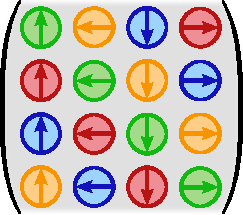
\includegraphics[width=.24\columnwidth]{figures/regular_C4_kernel.pdf}
    \captionsetup{width=1.1\columnwidth}
    \hspace{2ex}
    \caption{\small
        Degrees of freedom of a $\CN$-steerable kernel ${K: \R^2 \to \R^{N\times N}}$ which maps between feature fields that transform according to the regular representation ${\rho_{\textup{reg}}: \CN \to \GL{N}}$ for $N=4$~\cite{Weiler2019_E2CNN}.
        The kernel constraint, Eq.~\eqref{eq:kernel_constraint}, enforces the color-coded weight sharing pattern.
        The \mbox{PFCNNs} of \citet{Yang2020parallelFrameCNN} convolve features on each sheet of their $N$-direction field ($\CN$-structure) with rotated versions of a single scalar-valued kernel but do not include interaction between the different sheets.
        This shared kernel corresponds to the diagonal entries (green) of the complete kernel space.
        Off-diagonal entries, which are implicitly forced to zero, would correspond to interactions between the sheets.
        }
    \label{fig:regular_C4_kernel}
\end{SCfigure}

The feature spaces of PFCNNs are the spaces $C^\infty(\GM)$ of real-valued functions on $\GM$.
Since $\GM\!\xrightarrow{\piGM}\!M$ is for $G=\CN$ a $|G| = N$-fold cover of $M$, such feature fields can analogously be seen as assigning a tuple of $N$ real numbers to each point~$p\in M$.
As the $N$ sheets of the covering space are furthermore identified with $N$ directions (given by the first frame axes), these features are equivalent to the (discretized) directional functions of \citet{poulenard2018multi}.
Theorem~\ref{thm:regular_field_scalar_GM} in Appendix~\ref{apx:regular_field_scalar_GM} proves furthermore that there is an isomorphism
\begin{align}
    C^\infty(\GM)\ \cong\ \Gamma(\A_{\rho_\textup{reg}})
\end{align}
between the features of PFCNNs and our \emph{regular feature fields}.
PFCNNs are therefore performing coordinate independent convolutions between (an equivalent to) regular feature fields, and are thus identified as (specific) regular $\GM$-convolutions.

The formulation of parallel frame convolutions seems at first glance to be quite different from ours:
instead of convolving the full $N$-dimensional regular feature fields with a matrix-valued $\CN$-steerable kernel ${K: \R^2 \to \R^{N\times N}}$,
PFCNNs convolve their scalar functions on each of the $N$ sheets independently with a shared scalar-valued kernel which is aligned with the frame of the respective sheet.
This operation is in our framework interpreted as a convolution with a matrix-valued $\CN$-steerable kernel whose only non-zero values are on its diagonal and are rotated relative to each other, which is visualized by the green entries in Fig.~\ref{fig:regular_C4_kernel}.
The missing coupling between features on different sheets implies that the off-diagonal entries (yellow, blue and red) of the complete steerable kernel space are implicitly set to zero.
As already stated for MDGCNNs, the sparsity pattern of this regular $\GM$-convolution makes it computationally more efficient than a dense $\GM$-convolution but is likely to affect its performance and does not save memory cost.






\begin{figure}
    \centering
    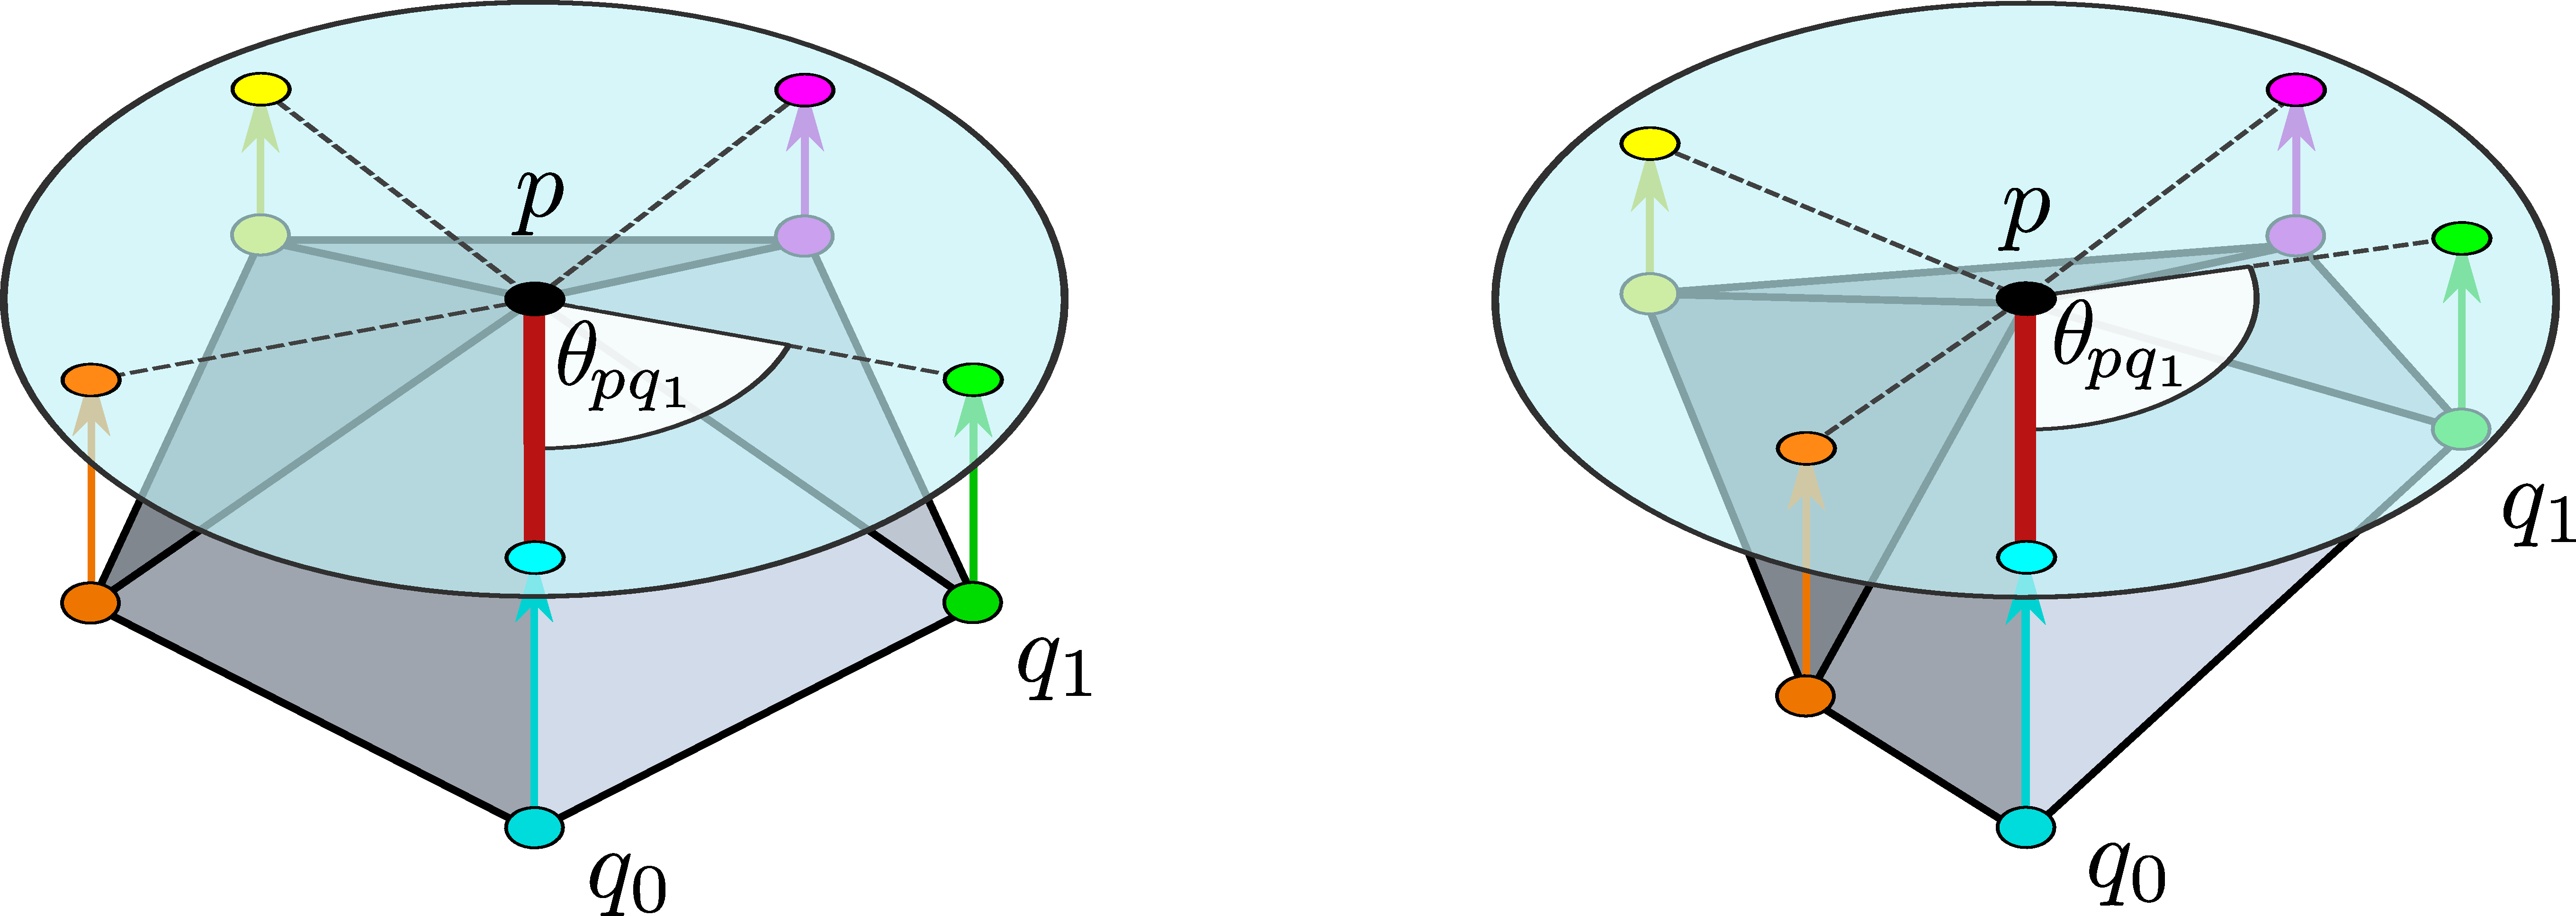
\includegraphics[width=.7\columnwidth]{figures/mesh_CNN_neighborhood_geometry.pdf}
    \vspace*{1ex}
    \caption{\small
        Two mesh regions which are topologically equivalent but geometrically distinct.
        One approach to define convolutions on meshes is to consider their underlying graph $(\mathcal{V},\mathcal{E})$, which captures the mesh topology, and run a graph neural network on it.
        Lacking information about the mesh geometry, (conventional) graph neural networks can not distinguish between the two visualized neighborhoods.
        Geometrically, they apply \emph{isotropic} kernels.
        The \emph{Gauge Equivariant Mesh CNNs} by \citet{deHaan2020meshCNNs} address this issue by projecting the neighboring vertices $q_i$ on the tangent planes and assigning them angles $\theta_{pq_i}$ relative to some reference edge, i.e. gauge (red).
        Requiring the coordinate independence of the convolutions leads to $G$-steerable kernels.
        While the model can discriminate based on the \emph{direction} of the neighboring nodes, it ignores their \emph{distance}.
        It furthermore deviates from our geodesic parametrization in that its kernel support is based on the local edge connectivity instead of geodesic distances.
        }
    \label{fig:mesh_CNNs_neighborhood}
\end{figure}


\paragraph{Gauge equivariant Mesh CNNs:}
The \emph{Gauge Equivariant Mesh CNN} (GEMCNN) by \citet{deHaan2020meshCNNs} is motivated by the shortcomings of conventional graph neural networks for the processing of feature fields on meshes.
Specifically, vanilla graph neural networks could be used to process vertex-sampled feature fields on meshes by convolving over the graph $(\mathcal{V},\mathcal{E})$ that is induced by the mesh.
The issue with this approach is that the graph encodes only the mesh \emph{topology}, but is not able to capture its \emph{geometry}.
Conventional graph convolutions do accordingly not distinguish between the ordering of edges, which corresponds on meshes to the use of \emph{isotropic kernels} that map between scalar fields.
Fig.~\ref{fig:mesh_CNNs_neighborhood} shows two regions of a mesh with distinct geometry but equivalent topology -- for conventional graph convolutions both neighborhoods look the same.
GEMCNNs address this issue by choosing a reference edge at each vertex $p\in\mathcal{V}$, relative to which the direction of all other edges $\{p,q_i\} \in\mathcal{E}$ to the one-ring of neighbors $q_i\in \mathcal{N}_p \subset\mathcal{V}$ is measured in terms of angles $\theta_{pq_i} \in [0,2\pi)$.
A choice of reference edge corresponds to a choice of orthonormal, right-handed frame.
Different choices are related by gauge transformations in the structure group~$G=\SO2$.

As in our theory, the feature spaces of GEMCNNs are defined as sections of associated vector bundles, i.e. as spaces of $c$-dimensional feature fields whose coefficients transform under gauge transformations according to some group representation $\rho: \SO2 \to \GL{c}$.
Each edge is assigned an $\SO2$-valued Levi-Civita transporter.
The convolution operation is demanded to be independent from the choice of reference edge, which leads to the requirement on the kernels to be $G$-steerable (gauge equivariant).
In contrast to our formulation, the kernels are not directly applied in geodesic normal coordinates but pass messages only from the one-ring neighborhoods $\mathcal{N}_p := \{q\in\mathcal{V} \,|\, \{p,q\}\in\mathcal{E} \}$ to that node~$p$ around which the kernel is centered.%
\footnote{
    For a (sufficiently) regular grid and compactly supported kernel in geodesic coordinates both approaches become equivalent.
}
The kernels are furthermore \emph{radially insensitive} --  in how far this affects the model performance remains an open question.

The authors decided for (real) \emph{irreps} as field types for the convolution, however, they perform a change of basis to \emph{regular representations} to apply ReLU nonlinearities, which is why we list them in row (38) of Table~\ref{tab:network_instantiations} instead of row (37).%
\footnote{
    The equivalence of $\rho$-fields to their \emph{irrep decomposition} was discussed in Section~\ref{sec:mobius_representations} and in Section~2.4 of~\cite{Weiler2019_E2CNN}.
}
Specifically, the authors use the change of basis $Q\in\R^{N\times N}$ that decomposes the regular representation $\rho_{\textup{reg}}: \CN \to \GL{N}$ of $\CN$ into its irrep components to transform a stack of irrep fields into one regular feature field.
For $\CN$, this matrix is just the discrete Fourier transform.
After applying the ReLU nonlinearity to each of the $N$ channels of the regular feature field individually -- which is a $\CN$-equivariant operation since regular representations are permutation representations -- the features are transformed back to a stack of irrep fields for the following convolution operation.
This design has the advantage that the features can be transported exactly with $\SO2$-valued transporters, without having to fall back to an interpolation scheme, as done by~\citet{poulenard2018multi}.
Note, however, that the full network is due to the use of the regular nonlinearities only $\CN$-equivariant.

That the authors use the \emph{real} irreps of $\SO2$ means that their kernel spaces are approximately twice as large as those of the Harmonic Surface Networks by \citet{Wiersma2020}; cf. the discussions in~\cite{Weiler2019_E2CNN,lang2020WignerEckart}.



\paragraph{Geodesic CNNs:}
The earliest work on geodesic convolutions that we are aware of is that of \citet{masci2015geodesic}.
The authors identified the rotational ambiguity of geodesic polar coordinates on an oriented Riemannian manifold and address it via a rotation \emph{invariant} architecture.
Their \emph{Geodesic convolutions} represent a \emph{scalar} field relative to arbitrarily oriented geodesic polar coordinates.
As the field type is trivial, the transporter pullback to geodesic coordinates does not require (non-trivial) transporters.
The feature field in geodesic coordinates is then matched with a scalar kernel, which is applied in $N$ equally spaced rotations by angles $\frac{2\pi}{N}k$ relative to the reference frame, where $k=0,\dots,N-1$.
Since a gauge transformation by $\frac{2\pi}{N}l$ for some $l\in\{0,\dots,N-1\}$ rotates all kernels accordingly, it result in a cyclic permutation of the responses by $l$ steps.
This operation corresponds therefore in our framework to a $\CN$-steerable convolution from scalar fields to $\CN$-regular feature fields.
Instead of processing these fields further via regular group convolutions
-- as done in MDGCNNs~\cite{poulenard2018multi}, PFCNNs~\cite{Yang2020parallelFrameCNN} and GEMCNNs~\cite{deHaan2020meshCNNs} --
the authors apply a $\max$-pooling operation over the $N$ responses.
Since $\CN$-valued gauge transformation result in cyclic shifts of the intermediate regular feature fields, the pooling operation is gauge-invariant, i.e. produces scalar fields.
While this networks design is simple to implement, it prevents features form encoding directional information.
Further variations of this networks design can be found in \cite{masci2015shapenet,monti2017geometric}.







\paragraph{ZerNet:}
Next, we turn to \emph{ZerNet} by \citet{sun2018zernet}.
To avoid confusion, we point out that the authors proposed two models, which we list in rows (38) \emph{and} (39) of Table~\ref{tab:network_instantiations}, respectively.
We describe both models, starting with their common design choices.

The key concept underlying ZerNets is their parameterization of convolution kernels in terms of \emph{Zernike polynomials}, which form an orthogonal basis of functions on the closed unit disk $B_{\R^2}(0,1)$ around the origin of $\R^2$.
In polar coordinates, Zernike polynomials are given by
\begin{alignat}{3}
    \textup{even:}\quad&&
        Z_n^m    &:\ [0,1]\times[0,2\pi) \to [-1,1], \quad (r,\varphi) \mapsto R_n^m(r)\, \cos(m\varphi)
        \qquad&& n\in\N,\ \ 0\leq m\leq n \\
    \textup{odd:}\quad&&
        Z_n^{-m} &:\ [0,1]\times[0,2\pi) \to [-1,1], \quad (r,\varphi) \mapsto R_n^m(r)\, \sin(m\varphi)
        \qquad&& n\in\N,\ \ 1\leq m\leq n \,,
\end{alignat}
where $R_n^m$ are the Zernike radial polynomials.
That (suitably normalized) Zernike polynomials are orthonormal means that they satisfy the orthonormality relations
\begin{align}
    \big\langle Z_n^m,\, Z_k^l \big\rangle_{B_{\R^2}(0,1)}
    \ =\ \int_0^1 \int_0^{2\pi} Z_n^m(r,\varphi)\, Z_k^l(r,\varphi)\ r\, dr\, d\varphi
    \ =\ \delta_{nk}\, \delta_{ml} \,.
\end{align}
A function on the unit disk, for instance a scalar kernel $K: B_{\R^2}(0,1) \to \R$, can be expanded in the Zernike polynomial basis:
\begin{align}
    K(r,\varphi)\ =\ \sum_{n\in\N}\, \sum_{m=-n}^n \widehat{K}_n^m\, Z_n^m(r,\varphi)
\end{align}
To retrieve the expansion coefficients of a given function on the unit disk, one projects it on the Zernike basis:
\begin{align}
    \widehat{K}_n^m
    \ =\ \big\langle K,\, Z_n^m \big\rangle_{B_{\R^2}(0,1)}
    \ =\ \int_0^1 \int_0^{2\pi} K(r,\varphi)\, Z_n^m(r,\varphi)\ r\, dr\, d\varphi
\end{align}
The inner product between two functions $K$ and $\Expspf^A$ on the unit disk can with these relations be expressed in terms of their expansion coefficients:
\begin{align}\label{eq:zernike_kernel_matching}
    \big\langle K,\, \Expspf^A \big\rangle_{B_{\R^2}(0,1)}
    \ =&\ \int_0^1 \int_0^{2\pi} K(r,\varphi)\, \Expspf^A(r,\varphi)\ r\, dr\, d\varphi \notag \\
    \ =&\ \int_0^1 \int_0^{2\pi}
        \sum_{n\in\N}\, \sum_{m=-n}^n \widehat{K}_n^m\, Z_n^m(r,\varphi)\,
        \sum_{k\in\N}\, \sum_{l=-k}^k \widehat{\big[\Expspf^A\big]}_k^l\, Z_k^l(r,\varphi)\ 
        r\, dr\, d\varphi \notag \\
    \ =&\ 
        \sum_{n\in\N}\, \sum_{m=-n}^n 
        \sum_{k\in\N}\, \sum_{l=-k}^k 
        \underbrace{\int_0^1 \int_0^{2\pi}\!
        Z_n^m(r,\varphi)\, Z_k^l(r,\varphi)\ 
        r\, dr\, d\varphi}_{\delta_{nk}\, \delta_{ml}}\ 
        \widehat{K}_n^m\, \widehat{\big[\Expspf^A\big]}_k^l \notag \\
    \ =&\ 
        \sum_{n\in\N}\, \sum_{m=-n}^n 
        \widehat{K}_n^m\, \widehat{\big[\Expspf^A\big]}_n^m
\end{align}
As suggested by the choices $K$ and $\Expspf^A$ for these functions, the authors use this property to match kernels with the pullback of the feature fields to geodesic polar coordinates.
The kernel coefficients $\widehat{K}_n^m$, which are set to zero beyond a user specified threshold, are optimized as learnable parameters of the network.
The expansion coefficients $\widehat{\big[\Expspf^A\big]}_n^m$ of the feature field's transporter pullback are computed by solving a linear system of equations.

An advantage of the kernel parameterization in terms of Zernike polynomials is that they are by definition \emph{$\SO2$-steerable kernels}.
Specifically, the pairs $\big(Z_n^m, Z_n^{-m}\big)^\top$ of kernels for a given $n\in\N$ and $1\leq m\leq n$ form a pair of kernels that are rotated by multiplying them with the $m$-th order real irrep of~$\SO2$,
\begin{align}
    \begin{pmatrix}
        Z_n^m \\ Z_n^{-m}
    \end{pmatrix}
    (r,\varphi + \Delta\varphi)
    \ =\ 
    \begin{pmatrix}
        \cos(m\Delta\varphi) &          -  \sin(m\Delta\varphi) \\
        \sin(m\Delta\varphi) & \phantom{-} \cos(m\Delta\varphi)
    \end{pmatrix}
    \begin{pmatrix}
        Z_n^m \\ Z_n^{-m}
    \end{pmatrix}
    (r,\varphi) \,,
\end{align}
while the kernels $Z_n^0$, i.e. for $m=0$, transform trivially (they are isotropic).
Note that the \emph{expansion coefficients} $\widehat{K}_n^m$ of a kernel $K$ transform \emph{inversely} to the basis.
The authors use this transformation law to rotate kernels analytically in terms of their expansion coefficients.
The rotation steerability of the Zernike polynomials' is independent from their radial parts but relies on the fact that their angular parts are \emph{circular harmonics}, which are the harmonic basis functions in the Peter-Weyl decomposition of $L^2(\SO2)$~\cite{lang2020WignerEckart}.
Due to their steerability properties, circular harmonic bases have been extensively used to parameterize real~\cite{Weiler2018SFCNN,graham2020dense} and complex~\cite{Worrall2017-HNET,Wiersma2020} convolution kernels since at least the '80s~\cite{Hsu1982optical,Rosen1988circularHarmonic,freeman1991design,hel1998canonical}.
In fact, circular harmonics are underlying \emph{any} $\SO2$-steerable kernel~\cite{Weiler2019_E2CNN,lang2020WignerEckart}.

The first and main model design described by \citet{sun2018zernet} is similar to that by~\citet{masci2015geodesic}.
A scalar field is pulled back to geodesic normal coordinates, where it is matched with a scalar kernel that is applied in $N$ discrete rotations, resulting in an intermediate $\CN$-regular feature field.
A subsequent $\max$-pooling operation over the $N$ responses yields then a $\CN$-invariant output, i.e. an output scalar field.
The difference to the implementation by \citet{masci2015geodesic} is that this operation is performed in the Zernike polynomial basis as specified in Eq.~\eqref{eq:zernike_kernel_matching}.
This choice corresponds ultimately to an alternative interpolation scheme.
The second model design, described Section~4.4 of~\cite{sun2018zernet}, is a reimplementation of the MDGCNNs from~\citet{poulenard2018multi} in the Zernike polynomial basis.
The authors observe that this design leads to a significantly improved performance since the regular feature fields are able to encode directional information.





\paragraph{TextureNet:}
The last rotation steerable model that we discuss is the \emph{TextureNet} by \citet{huang2019texturenet}.
\begin{wrapfigure}[13]{r}{0.22\textwidth}
    \centering
    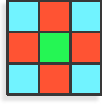
\includegraphics[width=.16\textwidth]{figures/3x3_D4_invariant_kernel.pdf}
    \captionsetup{width=.21\textwidth}
    \caption{\small
        \\
        A $\D4$-invariant kernel of $3\times3$ pixels is parameterized by three degrees of freedom.
        }
    \label{fig:3x3_D4_invariant_kernel}
\end{wrapfigure}%
In contrast to the previous models, TextureNets assume a $\D4$-structure, which could easily be generalized to a $\DN$-structure.
This $\D4$-structure is precomputed via QuadriFlow, a 3rd party software package which can be used to compute 4-RoSy fields that are optimized to be smooth and have few singularities~\cite{Huang2018QuadriFlow}.
As the name suggests, TextureNets process input feature fields that are represented as textures, and are of potentially higher resolution than the mesh.
The convolution kernels are applied at a dense set of sampling locations, which are uniformly distributed over the mesh's faces.
At each sampling point the scalar feature field is pulled back into geodesic normal coordinates and represented relative to an arbitrary frame of the $\D4$-structure.
It is then matched with a $\D4$-invariant $3\times3$ kernel.
As visualized in Fig.~\ref{fig:3x3_D4_invariant_kernel}, the 9 pixels of such kernels are described by 3 degrees of freedom.
The convolution is implemented in terms of three \onexones\ whose responses are subsequently binned and aggregated in each of the tangent spaces.
The additional reflection steerability of the kernels implies that TextureNets are well defined on non-orientable surfaces.
However, as the features of TextureNet are scalar fields they can neither encode directions nor orientations.
To overcome this issue, it is necessary to use non-trivial $\DN$ or $\O2$-steerable kernels.
